% F088｜algebra 原创简明教学示意图
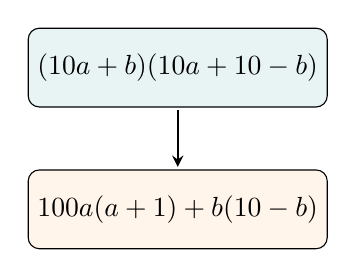
\begin{tikzpicture}[>=stealth,scale=.9]
\node[draw,fill=teal!9,rounded corners,minimum height=1cm] at (4,0){$(10a+b)(10a+10-b)$};
\draw[->,thick] (4,-.6)--(4,-1.4);
\node[draw,fill=orange!8,rounded corners,minimum height=1cm] at (4,-2){$100a(a+1)+b(10-b)$};
\end{tikzpicture}
